\documentclass[conference]{IEEEtran}

\PassOptionsToPackage{hyphens}{url}\usepackage[hidelinks]{hyperref}

\usepackage[dvipsnames,table,xcdraw]{xcolor}
\usepackage{tikz-inet, pgf, pgfplots}
\usepackage{tikzscale}
% \usepackage{url}
\usepackage{amsmath}
\usepackage{amssymb}
\usepackage{dsfont}
% \usepackage[breaklinks=true, colorlinks=true, linkcolor=blue, urlcolor=blue]{{hyperref}
\usepackage[capitalise]{cleveref}
\usepackage[acronym]{glossaries}
\usepackage{xspace}
\usepackage{algorithm}
\usepackage{algpseudocode}
\usepackage{graphicx}
\usepackage[caption=false]{subfig}
\usepackage{siunitx}
\usepackage{enumitem}
\usepackage{textcomp}
\usepackage{tabularx}
\usepackage{booktabs}
\usepackage{array}
\usepackage{multirow}
\usepackage{listings}
\usepackage{needspace}
\usepackage{caption}

%%%%%%%%%%%%%%%%%%%%%%%%%%%%%%%%%%%%%%%%%%%%%%%%%%%%%%%%%%%%%%%%%%%%%%%%%%%%%%%%%%%%%%%%%%%%%%%%%%%%%%%%

\usetikzlibrary{arrows, arrows.meta, automata, patterns, shapes, plotmarks, backgrounds, fit, positioning, shadows.blur, calc} %%
\usepgfplotslibrary{fillbetween, statistics, groupplots}
\pgfplotsset{compat=newest}

\pgfdeclarelayer{background}
\pgfsetlayers{background,main}

\DeclareSIUnit{\nothing}{\relax}
\DeclareSIUnit{\bit}{b}
\DeclareSIUnit{\Per}{/}
\DeclareSIUnit{\M}{M}
\DeclareSIUnit{\B}{B}
\sisetup{detect-weight=true, detect-family=true, group-separator = {,}}
\sisetup{per-mode=symbol, per-symbol = \text{p}}
% \sisetup{range-phrase = \text{--}}

% To enable Table Breaks
% \keepXColumns

% For code listings
\DeclareCaptionType{code}[Code][List of Codes]
\captionsetup[code]{labelsep=colon}

% For examples
\DeclareCaptionType{example}[Example][List of Examples]
\captionsetup[example]{labelsep=colon}

\crefname{code}{Code}{Codes}
\Crefname{code}{Code}{Codes}

\crefname{example}{Example}{Examples}
\Crefname{example}{Example}{Examples}
\definecolor{colorRed}{RGB}{199, 0, 11}
\definecolor{colorDarkGray}{RGB}{89, 87, 87}
\definecolor{colorGray}{RGB}{236, 236, 236}
\definecolor{colorGreen}{RGB}{98, 178, 48}
\definecolor{colorBlue}{RGB}{48, 181, 197}
\definecolor{colorOrange}{RGB}{237, 109, 0}
\definecolor{colorPurple}{rgb}{0.58, 0, 0.82}

%%%%%%%%%%%%%%%%%%%%%%%%%%%%%%%%%%%%%%%%%%%%%%%%%%%%%%%%%%%%%%%%%%%%%%%%%%%%%%%%%%%%%%%%%%%%%%%%%%%%%%%%
% Tikz colors
\colorlet{line1}{colorBlue}
\colorlet{line2}{colorOrange}
\colorlet{line3}{colorGreen}
\colorlet{line4}{colorDarkGray}
\definecolor{labelColor}{RGB}{85,85,85}
\definecolor{legendFillColor}{RGB}{229,229,229}
\definecolor{legendBorderColor}{RGB}{204 ,204, 204}
\colorlet{colorExtraGrid}{colorRed}

%%%%%%%%%%%%%%%%%%%%%%%%%%%%%%%%%%%%%%%%%%%%%%%%%%%%%%%%%%%%%%%%%%%%%%%%%%%%%%%%%%%%%%%%%%%%%%%%%%%%%%%%
% Code colors
\colorlet{delim}{red!60!black}
\colorlet{numb}{red!60!black}

% Table colors
\definecolor{tableGray}{gray}{0.98}
\newcommand{\tableColorBlock}[2]{\rowcolors{#1}{#2}{#2}}
\newcommand{\tableColors}{\rowcolors{2}{white}{tableGray}}
\newacronym{cdn}{CDN}{Content Delivery Network}
\newacronym{pop}{PoP}{Point-of-Presence}
\newacronym{sp}{SP}{Service Provider}
\newacronym{cp}{CP}{Content Provider}
\newacronym{cdnp}{CDN-P}{CDN Provider}
\newacronym{aip}{AIP}{AI Provider}
\newacronym{isp}{ISP}{Internet Service Provider}
\newacronym{ixp}{IXP}{Internet eXchange Point}

\newacronym{ecs}{ECS}{Edge Cache Server}
\newacronym{css}{CSS}{Content Steering Server}
\newacronym{sc}{SC}{Steering Controller}
\newacronym{mc3s2}{MC3S2}{Multi-CDN Communication over Content Steering Server}

%%%%%%%%%%%%%%%%%%%%%%% ORGANIZATIONS %%%%%%%%%%%%%%%%%%%%%%%
\newacronym{mpeg}{MPEG}{Moving Picture Experts Group}
\newacronym{dashif}{DASH\textendash IF}{DASH Industry Forum}
\newacronym{ict}{ICT}{Information Technology and Communication}
\newacronym{itu}{ITU}{International Telecommunication Union}
\newacronym{cta}{CTA}{Consumer Technology Association}
\newacronym{wave}{WAVE}{Web Application Video Ecosystem}
\newacronym{svta}{SVTA}{Streaming Video Technology Alliance}
\newacronym{eu}{EU}{European Union}
\newacronym{etsi}{ETSI}{European Telecommunications Standards Institute}
\newacronym{ietf}{IETF}{Internet Engineering Task Force}
\newacronym{iea}{IEA}{International Energy Agency}

%%%%%%%%%%%%%%%%%%%%%%% PROTOCOLS %%%%%%%%%%%%%%%%%%%%%%%
\newacronym{http}{HTTP}{Hypertext Transfer Protocol}
\newacronym{http2}{HTTP/2}{Hypertext Transfer Protocol Version 2}
\newacronym{http3}{HTTP/3}{Hypertext Transfer Protocol Version 3}
\newacronym{moq}{MoQ}{Media over QUIC}
\newacronym{quic}{QUIC}{Quick UDP Internet Connections}

\newacronym{udp}{UDP}{User Datagram Protocol}
\newacronym{tcp}{TCP}{Transmission Control Protocol}
\newacronym{dns}{DNS}{Domain Name System}
\newacronym{edns}{EDNS}{Extension Mechanisms for DNS}
\newacronym{nat}{NAT}{Network Address Translation}
\newacronym{bgp}{BGP}{Border Gateway Protocol}

\newacronym{webrtc}{WebRTC}{Web Real-Time Communications}
\newacronym{rtp}{RTP}{Real-time Transport Protocol}
\newacronym{rtcp}{RTCP}{RTP Control Protocol}
\newacronym{rtsp}{RTSP}{Real Time Streaming Protocol}
\newacronym{tls}{TLS}{Transport Layer Security}
\newacronym{srpt}{SRTP}{Secure Real-time Transport Protocol}
\newacronym{srt}{SRT}{Secure Reliable Transport}
\newacronym{rist}{RIST}{Reliable Internet Stream Transport}
\newacronym{rtmp}{RTMP}{Real-Time Messaging Protocol}
\newacronym{cdni}{CDNI}{Content Distribution Networks Interconnection}

%%%%%%%%%%%%%%%%%%%%%%% STREAMING PROTOCOLS %%%%%%%%%%%%%%%%%%%%%%%
\newacronym{hls}{HLS}{HTTP Live Streaming}
\newacronym{has}{HAS}{HTTP Adaptive Streaming}
\newacronym{dash}{DASH}{Dynamic Adaptive Streaming over HTTP}
\newacronym{llhls}{LL-HLS}{Low-Latency HLS}
\newacronym{lldash}{LL-DASH}{Low-Latency DASH}
\newacronym{mss}{MSS}{Microsoft Smooth Streaming}
\newacronym{ts}{MPEG-TS}{MPEG-2 Transport Stream}

\newacronym{cmcd}{CMCD}{Common Media Client Data}
\newacronym{cmsd}{CMSD}{Common Media Server Data}
\newacronym{cmaf}{CMAF}{Common Media Application Format}
\newacronym{abr}{ABR}{Adaptive Bitrate}
\newacronym{gop}{GOP}{Group of Pictures}
\newacronym{cbr}{CBR}{Constant Bitrate}
\newacronym{vbr}{VBR}{Variable Bitrate}
\newacronym{mse}{MSE}{Media Source Extensions}
\newacronym{isobmff}{ISOBMFF}{ISO Base Media File Format}

%%%%%%%%%%%%%%%%%%%%%%% STREAMING METRICS %%%%%%%%%%%%%%%%%%%%%%%
\newacronym{qoe}{QoE}{Quality of Experience}
\newacronym{qos}{QoS}{Quality of Service}
\newacronym{psnr}{PSNR}{Peak Signal-to-Noise Ratio}
\newacronym{ssim}{SSIM}{Structural Similarity Index}
\newacronym{vmaf}{VMAF}{Video Multimethod Assessment Fusion}

\newacronym{rtt}{RTT}{Round-Trip Time}
\newacronym{ttl}{TTL}{Time to Live}
\newacronym{lru}{LRU}{Least Recently Used}
\newacronym{lfu}{LFU}{Least Frequently Used}
\newacronym{gdsf}{GDSF}{Greedy Dual Size Frequency}
\newacronym{arc}{ARC}{Adaptive Replacement Cache}
\newacronym{hol}{HoL}{Head-of-Line}

%%%%%%%%%%%%%%%%%%%%%%% UNITS / MEASUREMENTS %%%%%%%%%%%%%%%%%%%%%%%
\newacronym{b}{B}{Byte}
\newacronym{kb}{KB}{KiloBytes}
\newacronym{mb}{MB}{MegaBytes}
\newacronym{gb}{GB}{GigaBytes}
\newacronym{w}{W}{Watt}
\newacronym{co}{CO\textsubscript{2}}{carbon dioxide}
\newacronym[longplural={Frames per Second}]{fpsLabel}{FPS}{Frame per Second}
\newacronym{pue}{PUE}{Power Usage Effectiveness}

%%%%%%%%%%%%%%%%%%%%%%% STREAMING MANIFEST %%%%%%%%%%%%%%%%%%%%%%%
\newacronym{dcsm}{DCSM}{DASH Content Steering Manifest}
\newacronym{hcsm}{HCSM}{HLS Content Steering Manifest}
\newacronym{m3u8}{M3U8}{UTF-8 M3U Playlist}
\newacronym{mpd}{MPD}{Media Presentation Description}
\newacronym{mvp}{MVP}{Multi Variant Playlist}

%%%%%%%%%%%%%%%%%%%%%%% CODEC %%%%%%%%%%%%%%%%%%%%%%%
\newacronym{avc}{AVC}{Advanced Video Coding (H.264)}
\newacronym{hevc}{HEVC}{High Efficiency Video Coding (H.265)}
\newacronym{vvc}{VVC}{Versatile Video Coding (H.266)}
\newacronym{av1}{AV1}{AOMedia Video 1}

\newacronym{hdr}{HDR}{High Dynamic Range}
\newacronym{uhd}{UHD}{Ultra-High-Definition}
\newacronym{hd}{HD}{High-Definition}
\newacronym{sd}{SD}{Standard-Definition}

\newacronym{url}{URL}{Uniform Resource Locator}
\newacronym{uri}{URI}{Uniform Resource Identifier}

\newacronym{dai}{DAI}{Dynamic Ad Insertion}
\newacronym{sgai}{SGAI}{Server-Guided Ad Insertion}
\newacronym{ssai}{SSAI}{Server-Side Ad Insertion}
\newacronym{csai}{CSAI}{Client-Side Ad Insertion}

\newacronym{sla}{SLA}{Service Level Agreement}
\newacronym{slo}{SLO}{Service Level Objective}
\newacronym{slis}{SLI}{Service Level Indicator}
\newacronym{lca}{LCA}{Life-Cycle Assessment}

\newacronym{api}{API}{Application Programming Interface}
\newacronym{poc}{PoC}{Proof of Concept}
\newacronym{sdk}{SDK}{Software Development Kit}
\newacronym{saas}{SaaS}{software-as-a-service}

\newacronym{ai}{AI}{Artificial Intelligence}
\newacronym{dl}{DL}{Deep Learning}
\newacronym{ml}{ML}{Machine Learning}
\newacronym{rl}{RL}{Reinforcement Learning}
\newacronym{drl}{DRL}{Deep Reinforcement Learning}

%%%%%%%%%%%%%%%%%%%%%%% SPEECH AND NLP %%%%%%%%%%%%%%%%%%%%%%%
\newacronym{asr}{ASR}{Automatic Speech Recognition}
\newacronym{llm}{LLM}{Large Language Model}
\newacronym{vad}{VAD}{Voice Activity Detection}
\newacronym{wer}{WER}{Word Error Rate}
\newacronym{nlp}{NLP}{Natural Language Processing}

%%%%%%%%%%%%%%%%%%%%%%% HARDWARE %%%%%%%%%%%%%%%%%%%%%%%
\newacronym{gpu}{GPU}{Graphic Processing Unit}
\newacronym{vram}{VRAM}{Video Random Access Memory}
\newacronym{nic}{NIC}{Network Interface Card}
\newacronym{cpu}{CPU}{Central Processing Unit}
\newacronym{asic}{ASIC}{Application-Specific Integrated Circuit}

\newacronym{drm}{DRM}{Digital Rights Management}
\newacronym{vod}{VOD}{Video on Demand}
\newacronym{live}{LIVE}{Live Linear Streaming}
\newacronym{ott}{OTT}{Over-The-Top}
\newacronym{voip}{VoIP}{Voice over IP}
\newacronym{iptv}{IPTV}{Internet Protocol Television}
\newacronym{ip}{IP}{Internet Protocol}

\newacronym{ghg}{GHG}{Greenhouse Gas}
\newacronym{dc}{DC}{Data Center}
\newacronym{vm}{VM}{Virtual Machine}
\newacronym{sdn}{SDN}{Software-Defined Networking}
\newacronym{ddos}{DDoS}{Distributed Denial-of-Service Attack}

\newacronym{de}{DE}{dirty energy}
\newacronym{ge}{GE}{green energy}

%%%%%%%%%%%%%%%%%%%%%%%%%%%%%%%%%%%%%%%%%%%%%%%%%%%%%%%%%%%%%%%%%%%%%%%%%%%%%%
\newacronym{idms}{IDMS}{Inter-Destination Media Synchronization}
\newacronym{av}{AV}{Audio/Video}

\newcommand{\ie}{\emph{i.e.}, }
\newcommand{\eg}{\emph{e.g.}, }
\newcommand{\etc}{\emph{etc.}\xspace}
\newcommand{\etal}{\emph{et al.} }
\newcommand{\td}{\textemdash}

%%%%%%%%%%%%%%%%%%%%%%%%%%%%%%%%%%%%%%%%%%%%%%%%%%%%%%%%%%%%%%%%%%%%%%%%%%%%%%%%%%%%%%%%%%%%%%%%%%%%%%%%

\newcommand\mc{\mathcal}
\def\cA {{\mathcal{A}}}
\def\cB {{\mathcal{B}}}
\def\cC {{\mathcal{C}}}
\def\cF {{\mathcal{F}}}
\def\cG {{\mathcal{G}}}
\def\cH {{\mathcal{H}}}
\def\cI {{\mathcal{I}}}
\def\cJ {{\mathcal{J}}}
\def\cL {{\mathcal{L}}}
\def\cO {{\mathcal{O}}}
\def\cP {{\mathcal{P}}}
\def\cR {{\mathcal{R}}}
\def\cS {{\mathcal{S}}}
\def\cT {{\mathcal{T}}}
\def\cU {{\mathcal{U}}}
\def\cV {{\mathcal{V}}}
\def\cX {{\mathcal{X}}}
\def\cY {{\mathcal{Y}}}
\newcommand{\E}{\mathds{E}}
\renewcommand{\P}{\mathds{P}}

%%%%%%%%%%%%%%%%%%%%%%%%%%%%%%%%%%%%%%%%%%%%%%%%%%%%%%%%%%%%%%%%%%%%%%%%%%%%%%%%%%%%%%%%%%%%%%%%%%%%%%%%

\newcommand{\quotes}[1]{``#1''\xspace}

%%%%%%%%%%%%%%%%%%%%%%%%%%%%%%%%%%%%%%%%%%%%%%%%%%%%%%%%%%%%%%%%%%%%%%%%%%%%%%%%%%%%%%%%%%%%%%%%%%%%%%%%

\newif\ifnotes\notesfalse
\def\boxnote#1#2{\ifnotes\fbox{\footnote{\ }}\ \footnotetext{From #1: #2}\fi}
\def\boxnoteh#1#2{\ifnotes\fbox{\footnote{\ }}\ \footnotetext{Removed by #1: #2}\fi}

\newcommand{\todo}[1]{{\color{red}TODO: #1}}
\def\burak#1{\boxnote{Burak}{\color{colorRed}#1}}
\newcommand{\mburak}[1]{{\color{colorGreen}#1}}

\newcommand{\ssection}[1]{%
    % \needspace{\baselineskip}%
     \vspace{0.6ex}%
    % \noindent\textbf{#1}\xspace%
  \noindent\textbf{#1}\xspace
}

\newcolumntype{L}{@{\extracolsep{\fill}}l}
\newcolumntype{R}{@{\extracolsep{\fill}}r}
\newcolumntype{C}{@{\extracolsep{\fill}}c}
\colorlet{line1}{colorBlue}
\colorlet{line2}{colorOrange}
\colorlet{line3}{colorGreen}
\colorlet{line4}{colorGray}

\def\ateachpoint{10}

\pgfplotscreateplotcyclelist{LineCycle}{%
    {line1, thick, mark=x, mark options={solid}, mark size = 2pt, mark repeat=75, filter discard warning=false, unbounded coords=discard},
    {line2, thick, densely dotted, mark=triangle, mark options={solid}, mark size = 1pt, mark repeat=75, filter discard warning=false, unbounded coords=discard},
    {line3, thick, densely dashed, mark=square, mark options={solid}, mark size = 1pt, mark repeat=75, filter discard warning=false, unbounded coords=discard},
    {line4, thick, thin, mark=Mercedes star, mark options={solid}, mark size = 4pt, mark repeat=70, each nth point={\ateachpoint}, filter discard warning=false, unbounded coords=discard},
    {line1, very thick, dashdotted, mark=x, mark options={solid}, mark size = 2pt, mark repeat=45, each nth point={\ateachpoint}, filter discard warning=false, unbounded coords=discard},
    {line2, very thick, dashdotted, mark=x, mark options={solid}, mark size = 2pt, mark repeat=45, each nth point={\ateachpoint}, filter discard warning=false, unbounded coords=discard}
}

\def\ateachpointLoose{30}
\pgfplotscreateplotcyclelist{LineCycleLoose}{%
    {line1, thick, mark=x, mark options={solid}, mark size = 4pt, mark repeat=15, each nth point={\ateachpointLoose}, filter discard warning=false, unbounded coords=discard},
    {line2, thick, densely dotted, mark=triangle, mark options={solid}, mark size = 2pt, mark repeat=17, each nth point={\ateachpointLoose}, filter discard warning=false, unbounded coords=discard},
    {line3, thick, densely dashed, mark=square, mark options={solid}, mark size = 2pt, mark repeat=19, each nth point={\ateachpointLoose}, filter discard warning=false, unbounded coords=discard},
    {line4, thick, thin, mark=Mercedes star, mark options={solid}, mark size = 2pt, mark repeat=16, each nth point={\ateachpointLoose}, filter discard warning=false, unbounded coords=discard},
    {line1, very thick, dashdotted, mark=x, mark options={solid}, mark size = 2pt, mark repeat=18, each nth point={\ateachpointLoose}, filter discard warning=false, unbounded coords=discard},
    {line2, very thick, dashdotted, mark=x, mark options={solid}, mark size = 2pt, mark repeat=15, each nth point={\ateachpointLoose}, filter discard warning=false, unbounded coords=discard}
}

\pgfplotsset{
    /pgfplots/area style/.style={%
        /pgfplots/cycle list={%
            {line1, mark=none, each nth point={\ateachpoint}},%
            {line2, mark=none, each nth point={\ateachpoint}},%
            {line3, mark=none, each nth point={\ateachpoint}},%
            {line4, mark=none, each nth point={\ateachpoint}}%
        }%
    }%
}%

\pgfplotsset{
   boxplot/every median/.style={ultra thick}
}

\pgfplotsset{
    compat=1.18,
    /pgfplots/boxplot legend/.style={
        /pgfplots/legend image code/.code={%
        \draw[##1,/tikz/.cd,yshift=-0.25em]
            (0cm,0cm) rectangle (6pt,6pt);},
    },
}

\pgfplotsset{
    compat=1.18,
	legend image code/.code={
		\draw[mark repeat=2, mark phase=2, rounded corners=2pt,]
		plot coordinates {
			(0cm,0cm)
			(0.15cm,0cm)        %% default is (0.3cm,0cm)
			(0.15cm,0cm)         %% default is (0.6cm,0cm)
		};%
	}
}

\pgfplotsset{
    every axis legend/.style={
        draw=legendBorderColor,
        fill=legendFillColor,
        fill opacity=0.1,
        text opacity=1,
        draw opacity=1, 
        legend columns=1,
        inner sep=2pt,
        /tikz/rounded corners=2pt,
    }
}

\pgfplotsset{
    every axis legend/.append style={
        legend pos=north east,
        legend cell align=left,
    }
}

\pgfplotsset{
    every axis/.style={
        tick align=inside,
        tick pos=both,
        tick style={line width=0.5pt, color=labelColor},
        tick label style={font=\small, color=labelColor},
        label style={font=\small, color=labelColor},
        title style={font=\small},
        legend style={font=\small, text={labelColor}},
        major grid style={dashed, labelColor},
        grid style=dashed,
        xminorgrids,
        yminorgrids,
        enlargelimits=0.05,
        clip=false,
        scaled ticks=false,
        axis line style={labelColor}
    }
}

\tikzstyle{every pin}=[
    labelColor,
    draw=legendBorderColor,
    fill=legendFillColor,
    font=\footnotesize,
    fill opacity=0.1,
    draw opacity=0.4,
    text opacity=1,
    pin distance = 1.6em,
    rounded corners=2pt, 
    inner sep=4pt,
    pin edge={labelColor, dashed, thin}
]

\tikzset{
    plotv/.style={
        domain=\ymin:\ymax,
        samples=2,
        thin,
        dash pattern=on 2pt off 8pt,
        color=labelColor
    },
    ploth/.style={
        domain=\xmin:\xmax,
        samples=2,
        thin,
        dash pattern=on 2pt off 8pt,
        color=labelColor
    },
}

%%%%%%%%%%%%%%%%%%%%%%%% not used yet %%%%%%%%%%%%%%%%%%%%%%%%

% \makeatletter
% \pgfplotsset{
%     boxplot prepared from table/.code={
%         \def\tikz@plot@handler{\pgfplotsplothandlerboxplotprepared}%
%         \pgfplotsset{
%             /pgfplots/boxplot prepared from table/.cd,
%             #1,
%         }
%     },
%     /pgfplots/boxplot prepared from table/.cd,
%         table/.code={\pgfplotstablecopy{#1}\to\boxplot@datatable},
%         row/.initial=0,
%         make style readable from table/.style={
%             #1/.code={
%                 \pgfplotstablegetelem{\pgfkeysvalueof{/pgfplots/boxplot prepared from table/row}}{##1}\of\boxplot@datatable
%                 \pgfplotsset{boxplot/#1/.expand once={\pgfplotsretval}}
%             }
%         },
%         make style readable from table=lower whisker,
%         make style readable from table=upper whisker,
%         make style readable from table=lower quartile,
%         make style readable from table=upper quartile,
%         make style readable from table=median,
%         make style readable from table=lower notch,
%         make style readable from table=upper notch
% }

% \makeatother
%     \pgfmathdeclarefunction{fpumod}{2}{%
%         \pgfmathfloatdivide{#1}{#2}%
%         \pgfmathfloatint{\pgfmathresult}%
%         \pgfmathfloatmultiply{\pgfmathresult}{#2}%
%         \pgfmathfloatsubtract{#1}{\pgfmathresult}%
%         % replaced `0' by `5' to make it work for this problem
%         \pgfmathfloatifapproxequalrel{\pgfmathresult}{#2}{\def\pgfmathresult{5}}{}%
%     }

% % defining the new dimensions and parameters
% \newlength{\hatchspread}
% \newlength{\hatchthickness}
% \newlength{\hatchshift}
% \newcommand{\hatchcolor}{}
% % declaring the keys in tikz
% \tikzset{
%     hatchspread/.code={\setlength{\hatchspread}{#1}},
%     hatchthickness/.code={\setlength{\hatchthickness}{#1}},
%     hatchshift/.code={\setlength{\hatchshift}{#1}},% must be >= 0
%     hatchcolor/.code={\renewcommand{\hatchcolor}{#1}}
% }
% % setting the default values
% \tikzset{
%     hatchspread=3pt,
%     hatchthickness=2pt,
%     hatchshift=0pt,% must be >= 0
%     hatchcolor=white
% }
         
% % declaring the pattern
% \pgfdeclarepatternformonly[\hatchspread,\hatchthickness,\hatchshift,\hatchcolor]% variables
%    {custom north west lines}% name
%    {\pgfqpoint{\dimexpr-2\hatchthickness}{\dimexpr-2\hatchthickness}}% lower left corner
%    {\pgfqpoint{\dimexpr\hatchspread+2\hatchthickness}{\dimexpr\hatchspread+2\hatchthickness}}% upper right corner
%    {\pgfqpoint{\dimexpr\hatchspread}{\dimexpr\hatchspread}}% tile size
%    {% shape description
%     \pgfsetlinewidth{\hatchthickness}
%     \pgfpathmoveto{\pgfqpoint{0pt}{\dimexpr\hatchspread+\hatchshift}}
%     \pgfpathlineto{\pgfqpoint{\dimexpr\hatchspread+0.15pt+\hatchshift}{-0.15pt}}
%     \ifdim \hatchshift > 0pt
%       \pgfpathmoveto{\pgfqpoint{0pt}{\hatchshift}}
%       \pgfpathlineto{\pgfqpoint{\dimexpr0.15pt+\hatchshift}{-0.15pt}}
%     \fi
%     \pgfsetstrokecolor{\hatchcolor}
% %    \pgfsetdash{{1pt}{1pt}}{0pt}% dashing cannot work correctly in all situation this way
%     \pgfusepath{stroke}
%    }

% \pgfdeclarepatternformonly[\hatchspread,\hatchthickness,\hatchshift,\hatchcolor]% variables
%    {custom north east lines}% name
%    {\pgfqpoint{\dimexpr-2\hatchthickness}{\dimexpr-2\hatchthickness}}% lower left corner
%    {\pgfqpoint{\dimexpr\hatchspread+2\hatchthickness}{\dimexpr\hatchspread+2\hatchthickness}}% upper right corner
%    {\pgfqpoint{\dimexpr\hatchspread}{\dimexpr\hatchspread}}% tile size
%    {% shape description
%     \pgfsetlinewidth{\hatchthickness}
%     \pgfpathmoveto{\pgfqpoint{\dimexpr\hatchshift-0.15pt}{-0.15pt}}
%     \pgfpathlineto{\pgfqpoint{\dimexpr\hatchspread+0.15pt}{\dimexpr\hatchspread-\hatchshift+0.15pt}}
%     \ifdim \hatchshift > 0pt
%       \pgfpathmoveto{\pgfqpoint{-0.15pt}{\dimexpr\hatchspread-\hatchshift-0.15pt}}
%       \pgfpathlineto{\pgfqpoint{\dimexpr\hatchshift+0.15pt}{\dimexpr\hatchspread+0.15pt}}
%     \fi
%     \pgfsetstrokecolor{\hatchcolor}
% %    \pgfsetdash{{1pt}{1pt}}{0pt}% dashing cannot work correctly in all situation this way
%     \pgfusepath{stroke}
%    }

% \pgfdeclarepatternformonly{mydots}
%     {\pgfqpoint{-1pt}{-1pt}}
%     {\pgfqpoint{1pt}{1pt}}
%     {\pgfqpoint{2pt}{2pt}}% original definition: \pgfqpoint{3pt}{3pt}
% {%
%   \pgfpathcircle{\pgfqpoint{0pt}{0pt}}{.8pt}%
%   \pgfusepath{fill}%
% }%

% % declaring the pattern
% \pgfdeclarepatternformonly%[\hatchspread,\hatchthickness,\hatchshift,\hatchcolor]% variables
%    {mynorthwestlines}% name
%    {\pgfqpoint{-4pt}{-4pt}}% lower left corner
%    {\pgfqpoint{8pt}{8pt}}% upper right corner
%    {\pgfqpoint{4pt}{4pt}}% tile size
%    {% shape description
%     \pgfsetlinewidth{2pt}
%     \pgfpathmoveto{\pgfqpoint{0pt}{4pt}}
%     \pgfpathlineto{\pgfqpoint{4.15pt}{-0.15pt}}
%     \pgfsetstrokecolor{white}
% %    \pgfsetdash{{1pt}{1pt}}{0pt}% dashing cannot work correctly in all situation this way
%     \pgfusepath{stroke}
%    }

% Style to select only points from #1 to #2 (inclusive)
% \pgfplotsset{select coords between index/.style 2 args={
%     x filter/.code={
%         \ifnum\coordindex<#1\def\pgfmathresult{}\fi
%         \ifnum\coordindex>#2\def\pgfmathresult{}\fi
%     }
% }}

% \newsavebox{\measuredSize}
% \newcommand{\resizeToWidth}[2]{%
%     \pgfmathsetmacro{\pgfplotswidth}{#2}%
%     \begin{lrbox}{\measuredSize}#1\end{lrbox}%
%     \pgfmathsetmacro{\pgfplotswidth}{2*\pgfplotswidth-\wd\measuredSize}%
%     #1%
% }

% \tikzset{every picture/.style={scale=1.4, transform shape}}

% \pgfplotsset{
%     discard if/.style 2 args={
%         x filter/.code={
%             \edef\tempa{\thisrow{#1}}
%             \edef\tempb{#2}
%             \ifx\tempa\tempb
%                 \def\pgfmathresult{inf}
%             \fi
%         }
%     },
%     discard if not/.style 2 args={
%         x filter/.code={
%             \edef\tempa{\thisrow{#1}}
%             \edef\tempb{#2}
%             \ifx\tempa\tempb
%             \else
%                 \def\pgfmathresult{inf}
%             \fi
%         }
%     }
% }

% \pgfplotscreateplotcyclelist{AreaCycle}{%
%     {line1, mark=none, pattern=crosshatch, pattern color = colorGray, each nth point={\ateachpoint}},
%     {line2, mark=none, pattern=mydots, pattern color = colorGreen, each nth point={\ateachpoint}},
%     {line3, mark=none, each nth point={\ateachpoint}},
%     {line4, mark=none, each nth point={\ateachpoint}}
% }



\def\BibTeX{{\rm B\kern-.05em{\sc i\kern-.025em b}\kern-.08em
    T\kern-.1667em\lower.7ex\hbox{E}\kern-.125emX}}

\begin{document}

\title{STREAMIND: A Real-Time AI Meeting Intelligence Pipeline}

\author{
    \IEEEauthorblockN{Mervegul Parlak, Alperen F. Zengin, \\Ayse B. Demir, Zafer Gurel, Ali C. Begen}
    \IEEEauthorblockA{
        \textit{Ozyegin University}\\
        Istanbul, Turkey}
    \and
    \IEEEauthorblockN{Burak Kara}
    \IEEEauthorblockA{
        \textit{Inria}\\
        Rennes, France}
}

\maketitle

\begin{abstract}
    \todo{Abstract: real-time meeting intelligence pipeline; scoring-formula-driven design; key contributions (streaming dedup, keyword guarantee, quality-gated latency optimisation); headline result.}
\end{abstract}

\begin{IEEEkeywords}
real-time speech processing, automatic speech recognition, large language models, streaming summarisation, WebRTC, Juturna
\end{IEEEkeywords}

% =====================================================================
\section{Introduction}
\label{sec:introduction}

\todo{Motivate live-audio intelligence (meetings, podcasts, IETF sessions). Frame the STREAMIND scoring formula $C_i = B_i + K_i + L_i$ with the $B_i \ge 10$ latency gate as the central design constraint: \emph{quality first, latency second, keyword discipline always}.}

\ssection{Contributions.}
\todo{Enumerate three contributions:
(1) streaming chunk deduplication that preserves temporal coherence across overlapping 5\,s ASR chunks while keeping the aggregated window non-redundant;
(2) a keyword guarantee algorithm that strips banned generic terms and back-fills missing slots from transcript proper nouns, converting the worst-case $-6$ LLM-failure mode into a $+0$ floor;
(3) quality-gated latency optimisation through prompt engineering and 4-bit quantisation, jointly cutting \texttt{proc\_time} by 24\,\% while keeping $B_i$ at ceiling.}

\ssection{Paper roadmap.}
\todo{Section ordering pointer.}

% =====================================================================
\section{Background and Related Work}
\label{sec:related}

\todo{Juturna node-graph framework. Janus WebRTC gateway. Streaming ASR: Whisper family, \texttt{faster-whisper} int8. LLM summarisation under latency constraints; small-model 4-bit quantisation (Qwen3.5 OptiQ). Position STREAMIND as a \emph{systems} contribution wrapping these primitives, not a new model.}

% =====================================================================
\section{System Architecture}
\label{sec:architecture}

\todo{High-level pipeline overview: insert Figure~\ref{fig:pipeline}. Explain seven-stage data flow from Opus/RTP ingestion to challenge-endpoint POST. State the scoring-aware design principle: every component is justified against one or more terms of $C_i = B_i + K_i + L_i$.}

\begin{figure*}[t]
    \centering
    % F1 — STREAMIND pipeline architecture block diagram.
% Eight Juturna nodes from Janus ingestion to challenge-endpoint POST.
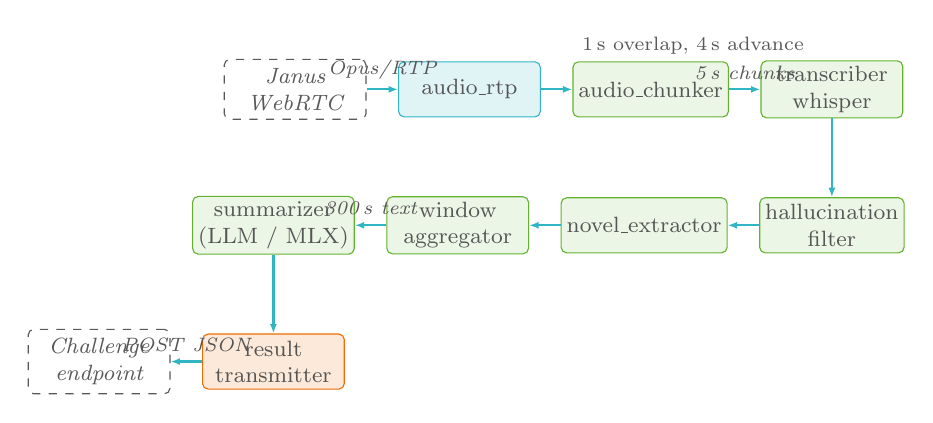
\begin{tikzpicture}[
    every node/.style={font=\footnotesize},
    node distance=4mm and 4mm,
    block/.style={
        draw=labelColor, fill=legendFillColor, rounded corners=2pt,
        minimum width=18mm, minimum height=7mm, align=center, inner sep=2pt,
        text=labelColor
    },
    source/.style={block, fill=colorBlue!15, draw=colorBlue},
    proc/.style={block, fill=colorGreen!12, draw=colorGreen},
    sink/.style={block, fill=colorOrange!15, draw=colorOrange},
    external/.style={
        draw=colorDarkGray, dashed, rounded corners=2pt,
        minimum width=18mm, minimum height=7mm, align=center,
        font=\footnotesize\itshape, text=colorDarkGray
    },
    arrow/.style={-{Latex[length=1.2mm]}, line1, thick},
    label-edge/.style={font=\scriptsize\itshape, text=labelColor, midway, above, sloped}
]
    \node[external] (janus) {Janus\\WebRTC};
    \node[source, right=of janus] (rtp) {audio\_rtp};
    \node[proc, right=of rtp] (chunker) {audio\_chunker};
    \node[proc, right=of chunker] (asr) {transcriber\\whisper};

    \node[proc, below=10mm of asr] (halluc) {hallucination\\filter};
    \node[proc, left=of halluc] (novel) {novel\_extractor};
    \node[proc, left=of novel] (window) {window\\aggregator};
    \node[proc, left=of window] (summ) {summarizer\\(LLM / MLX)};

    \node[sink, below=10mm of summ] (sink) {result\\transmitter};
    \node[external, left=of sink] (endpoint) {Challenge\\endpoint};

    \draw[arrow] (janus) -- node[label-edge]{Opus/RTP} (rtp);
    \draw[arrow] (rtp) -- (chunker);
    \draw[arrow] (chunker) -- node[label-edge]{5\,s chunks} (asr);
    \draw[arrow] (asr.south) -- ++(0,-3mm) -| (halluc.north);
    \draw[arrow] (halluc) -- (novel);
    \draw[arrow] (novel) -- (window);
    \draw[arrow] (window) -- node[label-edge]{300\,s text} (summ);
    \draw[arrow] (summ.south) -- ++(0,-3mm) -| (sink.north);
    \draw[arrow] (sink) -- node[label-edge]{POST JSON} (endpoint);

    \node[font=\scriptsize, text=colorDarkGray, anchor=west]
        at ([yshift=2mm]chunker.north west) {1\,s overlap, 4\,s advance};
\end{tikzpicture}

    \caption{End-to-end STREAMIND pipeline. Janus delivers mono Opus/RTP into \texttt{audio\_rtp}; chunks slide every 4\,s through ASR; deduplication and hallucination filtering precede a 300\,s aggregation buffer; the summariser emits \texttt{\{summary, keywords[3]\}} per window; the sink stores locally and POSTs to the challenge endpoint.}
    \label{fig:pipeline}
\end{figure*}

\begin{figure}[t]
    \centering
    % F2 — Latency bonus L_i = 10 * exp(-0.5 * proc_time), gated by B_i >= 10.
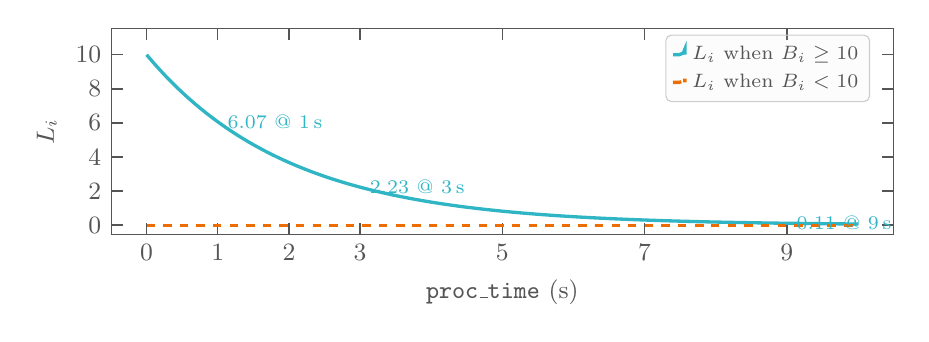
\begin{tikzpicture}
    \begin{axis}[
        width=0.95\columnwidth,
        height=4.2cm,
        xlabel={\texttt{proc\_time} (s)},
        ylabel={$L_i$},
        xmin=0, xmax=10,
        ymin=0, ymax=11,
        domain=0:10,
        samples=120,
        ytick={0, 2, 4, 6, 8, 10},
        xtick={0, 1, 2, 3, 5, 7, 9},
        legend pos=north east,
        legend style={font=\scriptsize, inner sep=2pt},
    ]
        \addplot[line1, very thick, no marks] {10 * exp(-0.5 * x)};
        \addlegendentry{$L_i$ when $B_i \ge 10$}

        \addplot[line2, very thick, dashed, no marks, domain=0:10] {0};
        \addlegendentry{$L_i$ when $B_i < 10$}

        \node[anchor=west, font=\scriptsize, text=line1]
            at (axis cs:1, {10*exp(-0.5)}) {6.07 @ 1\,s};
        \node[anchor=west, font=\scriptsize, text=line1]
            at (axis cs:3, {10*exp(-1.5)}) {2.23 @ 3\,s};
        \node[anchor=west, font=\scriptsize, text=line1]
            at (axis cs:9, {10*exp(-4.5)}) {0.11 @ 9\,s};
    \end{axis}
\end{tikzpicture}

    \caption{Latency bonus $L_i = 10 e^{-0.5 \cdot \mathrm{proc\_time}}$, gated by $B_i \ge 10$. Below the gate, latency contributes zero; above it, returns diminish past $\sim$1--2\,s.}
    \label{fig:scoring}
\end{figure}

\subsection{Audio Reception}
\label{sec:arch:audio}
\todo{Janus WebRTC gateway forwards mono Opus/48k as RTP to \texttt{audio\_rtp} on UDP/8888. Identical code paths in dev and eval environments; earns the flat $+4$ audio-level Janus bonus. Cite Janus.}

\subsection{Incremental ASR}
\label{sec:arch:asr}
\todo{\texttt{audio\_chunker} buffers the stream into 5\,s chunks with 1\,s overlap (advance = 4\,s) so the ASR sees audio incrementally. \texttt{transcriber\_whisper} runs \texttt{faster-whisper} \texttt{small.en} (int8, \texttt{device: auto}). VAD filter enabled; previous-text conditioning disabled to avoid context drift.}

\subsection{Hallucination Filter}
\label{sec:arch:halluc}
\todo{Post-ASR guard. Strips Whisper noise tags (\texttt{[Music]}, \texttt{(applause)}) and drops pure-hallucination outputs against a configurable exact-match block-list. Protects $B_i$ factual-consistency. Insert Figure~\ref{fig:chunk-overlap} here or in §\ref{sec:arch:novel}.}

\subsection{Novel Chunk Extraction}
\label{sec:arch:novel}
\todo{Word-level overlap detection: longest suffix-prefix match up to \texttt{max\_overlap\_words}\,=\,10 with a \texttt{SequenceMatcher} fallback (\texttt{similarity\_threshold}\,=\,0.8). Emits only novel words. Preserves temporal coherence across overlapping ASR chunks; prevents duplicate content reaching the aggregator. Refer to Figure~\ref{fig:chunk-overlap}.}

\begin{figure}[t]
    \centering
    % F3 — Chunking + novel-extraction timing diagram.
% Five-second chunks slide every 4 s; novel extractor isolates the new 4 s
% per step (drops the 1 s of overlap with the previous chunk).
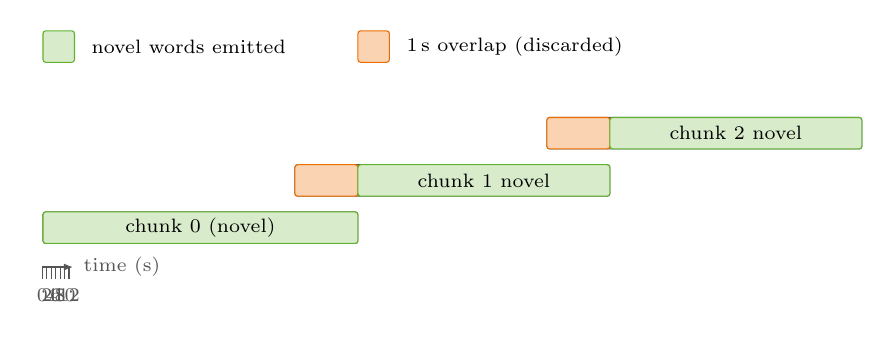
\begin{tikzpicture}[
    every node/.style={font=\scriptsize},
    chunk/.style={
        draw=labelColor, fill=colorBlue!12, rounded corners=1pt,
        minimum height=4mm, anchor=west, inner sep=0pt
    },
    overlap/.style={
        draw=colorOrange, fill=colorOrange!30, rounded corners=1pt,
        minimum height=4mm, anchor=west, inner sep=0pt
    },
    novel/.style={
        draw=colorGreen, fill=colorGreen!25, rounded corners=1pt,
        minimum height=4mm, anchor=west, inner sep=0pt
    },
    axis-style/.style={-{Latex[length=1.2mm]}, thick, color=labelColor},
    tick-style/.style={color=labelColor, font=\scriptsize}
]
    % Time axis: 1 unit = 8 mm, total 14 s.
    \def\u{8mm}
    \draw[axis-style] (0,0) -- (14*\u/1cm,0) node[right]{time (s)};
    \foreach \t in {0,2,4,6,8,10,12}{
        \draw[tick-style] (\t*\u/1cm,0) -- (\t*\u/1cm,-1.5mm) node[below]{\t};
    }

    % Chunk 0: [0, 5]
    \node[chunk, minimum width=5*\u] at (0,5mm) {};
    \node[novel, minimum width=5*\u] at (0,5mm) {chunk 0 (novel)};

    % Chunk 1: [4, 9], overlap [4,5] with previous
    \node[chunk, minimum width=5*\u] at (4*\u,11mm) {};
    \node[overlap, minimum width=1*\u] at (4*\u,11mm) {};
    \node[novel, minimum width=4*\u] at (5*\u,11mm) {chunk 1 novel};

    % Chunk 2: [8, 13], overlap [8,9]
    \node[chunk, minimum width=5*\u] at (8*\u,17mm) {};
    \node[overlap, minimum width=1*\u] at (8*\u,17mm) {};
    \node[novel, minimum width=4*\u] at (9*\u,17mm) {chunk 2 novel};

    % Legend.
    \node[novel, minimum width=4mm] at (0,28mm) {};
    \node[anchor=west] at (5mm,28mm) {novel words emitted};
    \node[overlap, minimum width=4mm] at (40mm,28mm) {};
    \node[anchor=west] at (45mm,28mm) {1\,s overlap (discarded)};
\end{tikzpicture}

    \caption{Audio chunking and novel extraction timing. Five-second chunks slide by 4\,s; the novel extractor isolates the 4\,s of newly-spoken content each step, dropping the 1\,s of overlap with the previous chunk.}
    \label{fig:chunk-overlap}
\end{figure}

\subsection{Window Aggregation}
\label{sec:arch:window}
\todo{\texttt{window\_aggregator} concatenates novel transcript segments into a rolling 300\,s context window. Flush trigger: \texttt{chunk\_end} $\ge$ \texttt{window\_start} $+$ 300\,s. Graceful stop emits partial windows on pipeline shutdown.}

\subsection{Summarisation}
\label{sec:arch:summ}
\todo{Two interchangeable backends with identical output schema: \texttt{summarizer\_llm} (Ollama, Qwen3.5-4B, CUDA target) and \texttt{summarizer\_mlx} (MLX, Qwen3.5 2B/4B/9B OptiQ-4bit, Apple Silicon dev). Prompt engineering for conciseness + specificity (1--2 sentences, specific noun-phrase keywords) double-up: higher $B_i$ conciseness score and lower \texttt{num\_predict}, which boosts $L_i$. \texttt{/no\_think} flag suppresses chain-of-thought. Robust output cleaning strips ChatML tokens (\texttt{<|im\_end|>}, \texttt{<|endoftext|>}) and extracts the outermost balanced JSON object.}

\subsection{Keyword Validation}
\label{sec:arch:keywords}
\todo{Shared \texttt{ensure\_three\_keywords} (\texttt{plugins/nodes/proc/\_summarizer\_common/keywords.py}) guarantees exactly three keywords regardless of LLM output state. Pipeline: (i) deduplicate case-insensitively, (ii) drop banned generic terms (\quotes{general}, \quotes{discussion}, \quotes{meeting}), (iii) back-fill from transcript by frequency + capitalisation ranking, (iv) pad with conservative fallbacks. Converts $-6$ worst-case into $+0$ floor.}

\subsection{Result Transmission}
\label{sec:arch:sink}
\todo{\texttt{result\_transmitter} maps internal keys to challenge contract (\texttt{window\_start} $\to$ \texttt{from}, \texttt{window\_end} $\to$ \texttt{to}, \texttt{latency} $\to$ \texttt{proc\_time}), writes \texttt{results/\{model\}/\{window\}/window\_N.json}, and POSTs to \texttt{destination\_endpoint} when configured. Drains pending messages on stop.}

% =====================================================================
\section{Implementation and Deployment}
\label{sec:implementation}

\todo{Pipeline-config assembly: \texttt{tools/assemble\_config.py} merges \texttt{config-base.json} with a summariser profile JSON. Launcher: \texttt{tools/run\_pipeline.sh}.}

\todo{Single-image Docker submission: CUDA 12.3 runtime, Python 3.12 + \texttt{uv}, Ollama daemon, pre-pulled Qwen3.5-4B baked at build time. \texttt{docker-compose.yml} orchestrates Janus + pipeline. Entry point starts Ollama, waits for readiness, then launches the pipeline with the submission profile.}

\todo{Reproducibility checklist: dataset hashes, model revision pins, RTP \texttt{payload\_type}, \texttt{encoding\_clock\_chan}.}

\begin{table}[t]
    \centering
    \caption{Pipeline nodes (Juturna).}
    \label{tab:nodes}
    \todo{Rows: \texttt{audio\_rtp}, \texttt{audio\_chunker}, \texttt{transcriber\_whisper}, \texttt{hallucination\_filter}, \texttt{novel\_extractor}, \texttt{window\_aggregator}, \texttt{summarizer\_llm}/\texttt{summarizer\_mlx}, \texttt{result\_transmitter}. Columns: type, model/algorithm, key hyper-parameters, role.}
\end{table}

\begin{table}[t]
    \centering
    \caption{Summariser profiles.}
    \label{tab:profiles}
    \todo{Columns: profile, backend, model, quantisation, temp, top\_p, repetition\_penalty, mem footprint, target hardware. Rows: ollama-qwen3.5-4b (submission default, CUDA), ollama-qwen3.5-9b, mlx-Qwen3.5-2B-OptiQ-4bit, mlx-Qwen3.5-4B-OptiQ-4bit, mlx-Qwen3.5-9B-OptiQ-4bit.}
\end{table}

% =====================================================================
\section{Evaluation}
\label{sec:evaluation}

\subsection{Setup}
\label{sec:eval:setup}
\todo{Datasets: \texttt{youtube\_15min.wav} 120\,s slice (≥3 full 300\,s windows); secondary against the \texttt{rev16} Whisper subset (30 podcast episodes) and \texttt{ietf} IETF125 sessions. Judge harness: \texttt{tools/eval\_quality.py} with local \texttt{qwen3.5:9b-16k} as judge. Disclose: this approximates the official judge; numbers are directional. Hardware: Apple Silicon M-series (MLX, dev); NVIDIA RTX 4090 dev box and RTX Pro 4500 target (CUDA, Ollama).}

\subsection{End-to-End Scoring}
\label{sec:eval:scoring}
\todo{Per-window $B_i / K_i / L_i / C_i$ and audio-level mean across summariser profiles. Refer to Table~\ref{tab:per-window}.}

\begin{table}[t]
    \centering
    \caption{Per-window scores on \texttt{youtube\_15min.wav}, 300\,s windows, Qwen3.5-4B (CUDA).}
    \label{tab:per-window}
    \todo{Columns: window, from (s), to (s), proc\_time (s), $B_i$, $K_i$, $L_i$, $C_i$. Numbers TBD from CUDA bench.}
\end{table}

\subsection{Latency Profile}
\label{sec:eval:latency}
\todo{\texttt{proc\_time} distribution; refer to Figure~\ref{fig:scoring} for the $L_i$ curve. Optional per-stage breakdown (ASR vs LLM) if instrumentation lands.}

\subsection{Ablations}
\label{sec:eval:ablation}
\todo{Four single-component removals plus the Phase-1 fix package. See Figure~\ref{fig:phase1-ablation} and Table~\ref{tab:ablation}.}

\begin{figure}[t]
    \centering
    % F4 — Phase-1 ablation: three side-by-side panels via groupplots so each
% metric uses its own y-axis. Numbers are MLX 4B on 30 s windows of
% youtube_15min.wav (docs/APPROACH.md). CUDA target-hardware numbers will
% overlay once the bench lands.
\def\panelW{0.30\columnwidth}
\def\panelH{3.6cm}
\def\barW{12pt}

\pgfmathsetmacro{\procPre}{4.09}
\pgfmathsetmacro{\procPost}{3.10}
\pgfmathsetmacro{\LPre}{1.34}
\pgfmathsetmacro{\LPost}{2.13}
\pgfmathsetmacro{\CPre}{32.06}
\pgfmathsetmacro{\CPost}{33.13}

\begin{tikzpicture}
    \begin{groupplot}[
        group style={
            group size=3 by 1,
            horizontal sep=10mm,
        },
        width=\panelW, height=\panelH,
        ybar,
        /pgf/bar width=\barW,
        enlargelimits=0.45,
        symbolic x coords={Pre, Post},
        xtick=data,
        ymin=0,
        nodes near coords,
        nodes near coords style={
            font=\tiny,
            text=labelColor,
            /pgf/number format/.cd, fixed, precision=2, /tikz/.cd
        },
        every node near coord/.append style={anchor=south},
        xticklabel style={font=\scriptsize, text=labelColor},
        yticklabel style={font=\scriptsize, text=labelColor},
        ylabel style={font=\scriptsize, text=labelColor},
        title style={font=\scriptsize, text=labelColor},
        axis lines=left,
        axis line style={color=labelColor},
        grid=major,
        major grid style={dashed, line4!25},
    ]
        \nextgroupplot[
            title={\texttt{proc\_time} (s)},
            ymax=5.2,
        ]
        \addplot[fill=line2!55, draw=line2!85]
            coordinates {(Pre, \procPre)};
        \addplot[fill=line1!65, draw=line1!85]
            coordinates {(Post, \procPost)};

        \nextgroupplot[
            title={$L_i$},
            ymax=2.8,
        ]
        \addplot[fill=line2!55, draw=line2!85]
            coordinates {(Pre, \LPre)};
        \addplot[fill=line1!65, draw=line1!85]
            coordinates {(Post, \LPost)};

        \nextgroupplot[
            title={$C_i$},
            ymin=30, ymax=34.5,
            ytick={30, 31, 32, 33, 34},
        ]
        \addplot[fill=line2!55, draw=line2!85]
            coordinates {(Pre, \CPre)};
        \addplot[fill=line1!65, draw=line1!85]
            coordinates {(Post, \CPost)};
    \end{groupplot}

    % Shared legend below the three panels.
    \node[
        anchor=north,
        font=\scriptsize,
        text=labelColor,
        draw=line4!60, fill=legendFillColor!30,
        rounded corners=2pt, inner sep=3pt,
        below=4mm of group c2r1.south
    ] {%
        \textcolor{line2!75!black}{$\blacksquare$} Pre-Phase-1
        \hspace{6mm}
        \textcolor{line1!75!black}{$\blacksquare$} Post-Phase-1%
    };
\end{tikzpicture}

    \caption{Phase-1 ablation. Pre-Phase-1 vs Post-Phase-1 \texttt{proc\_time}, $L_i$, and $C_i$ on 30\,s windows of \texttt{youtube\_15min.wav}. Phase-1 fixes (prompt tightening, \texttt{num\_predict\,=\,150}, banned-keyword filter, JSON extraction fix) cut \texttt{proc\_time} 24\,\% and lifted $L_i$ 59\,\% while holding $B_i$ at ceiling.}
    \label{fig:phase1-ablation}
\end{figure}

\begin{table}[t]
    \centering
    \caption{Component ablation. $\Delta$ relative to the full pipeline.}
    \label{tab:ablation}
    \todo{Rows: baseline (full pipeline), $-$banned\_keywords, $-$hallucination\_filter, $-$novel\_extractor. Columns: $\Delta B_i$, $\Delta K_i$, $\Delta L_i$, $\Delta C_i$. Numbers TBD from CUDA bench.}
\end{table}

\subsection{Model-Size Sweep}
\label{sec:eval:sweep}
\todo{Qwen3.5 2B vs 4B vs 9B. MLX (Apple Silicon) and CUDA (Ollama, RTX Pro 4500). See Figure~\ref{fig:model-sweep}.}

\begin{figure}[t]
    \centering
    % F5 — Final source score (avg C + 4 Janus bonus) for Qwen3.5 model variants.
% Data: cross-audio mean ± std across 3 Rev16 episodes, 300 s windows, RTX 4090.
% 4B-AWQ: 40.14±0.85 | 4B-BF16: 38.97±0.91 | 9B-AWQ: 37.15±1.53 | 9B-BF16: 36.12±1.42
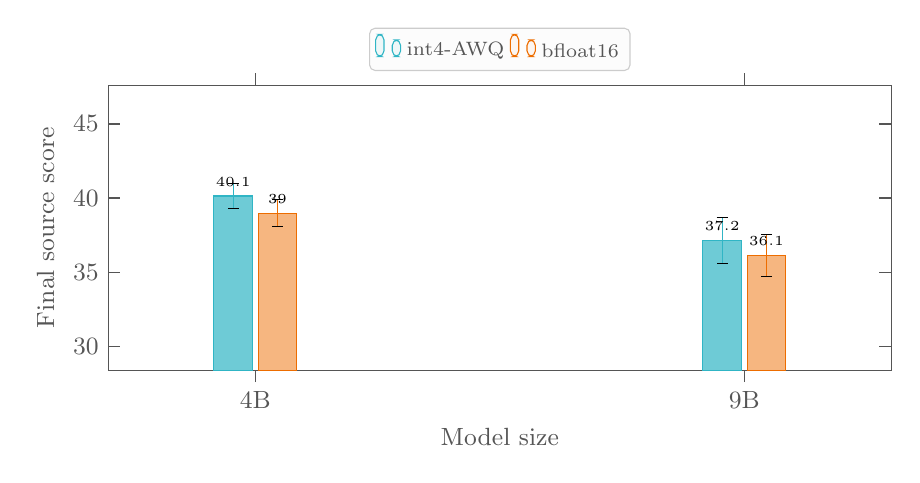
\begin{tikzpicture}
    \begin{axis}[
        width=0.95\columnwidth,
        height=5.2cm,
        ybar=2pt,
        bar width=14pt,
        enlargelimits=0.3,
        ylabel={Final source score},
        symbolic x coords={4B, 9B},
        xtick=data,
        xlabel={Model size},
        nodes near coords,
        nodes near coords style={font=\tiny, /pgf/number format/.cd, fixed, precision=1, /tikz/.cd},
        ymin=32, ymax=44,
        legend style={
            at={(0.5,1.05)}, anchor=south, legend columns=-1,
            font=\scriptsize, inner sep=2pt,
        },
        error bars/y dir=both,
        error bars/y explicit,
    ]
        \addplot[fill=line1!70, draw=line1] plot [error bars/.cd, y dir=both, y explicit]
        coordinates {
            (4B, 40.14) +- (0, 0.85)
            (9B, 37.15) +- (0, 1.53)
        };
        \addlegendentry{int4-AWQ}

        \addplot[fill=line2!50, draw=line2] plot [error bars/.cd, y dir=both, y explicit]
        coordinates {
            (4B, 38.97) +- (0, 0.91)
            (9B, 36.12) +- (0, 1.42)
        };
        \addlegendentry{bfloat16}
    \end{axis}
\end{tikzpicture}

    \caption{Quality vs latency across Qwen3.5 model sizes (2B/4B/9B) on MLX (Apple Silicon) and Ollama (RTX Pro 4500). Larger models trade \texttt{proc\_time} for marginal $B_i$ gains; the gate at $B_i \ge 10$ makes the sweet spot model-size-dependent.}
    \label{fig:model-sweep}
\end{figure}

\subsection{Threats to Validity}
\label{sec:eval:threats}
\todo{Local judge $\ne$ official judge; held-out audio is small; deterministic decoding settings; eval hardware availability.}

% =====================================================================
\section{Discussion}
\label{sec:discussion}

\todo{What the scoring formula encourages vs what real users want (gist coherence over keyword precision; latency only matters once quality clears the gate). Limits of static prompt tuning. Future work: per-window adaptive prompts, speculative decoding, batched ASR, structured-output decoding.}

% =====================================================================
\section{Conclusion}
\label{sec:conclusion}

\todo{Recap three contributions. State final claimed audio-level score (avg $C_i$ + 4 Janus bonus) on the submission profile. Point at the open-source release.}

% =====================================================================
\bibliographystyle{IEEEtran}
\bibliography{references}

\end{document}
